\documentclass{article}

\usepackage[utf8]{inputenc}
\usepackage{amsmath}
\usepackage{graphicx}
\usepackage{float}
%package for images
\usepackage{graphicx}


\title{Ecommerce Backend}
\author{Mohamad Lakkis}
\date{\today}

\begin{document}

\maketitle

\begin{abstract}
abstract, I will write it later.
\end{abstract}

\section{Installing required packages}
\begin{figure}[H]
\centering
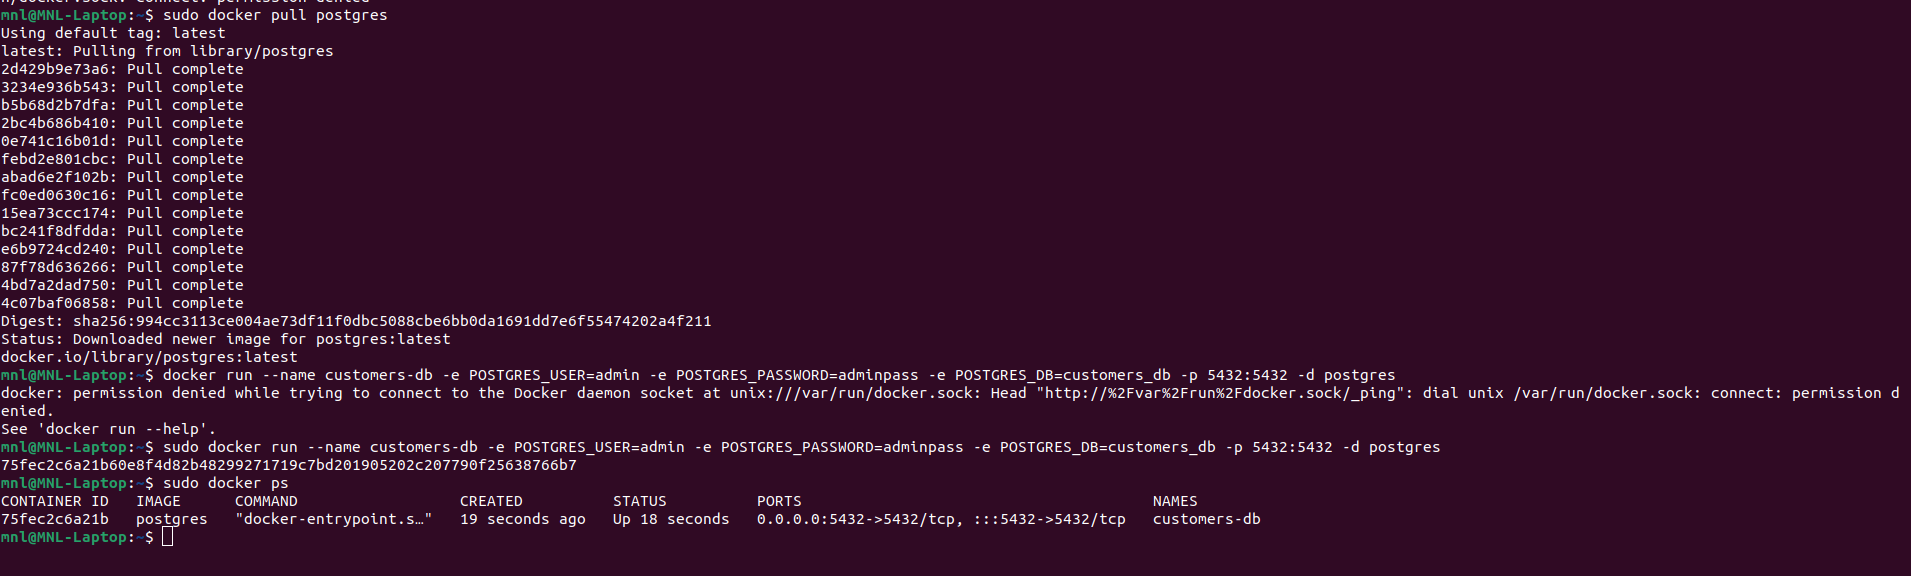
\includegraphics[width=0.9\textwidth]{images/1.png}
\caption{Installing postgreSQL image from docker hub, and running it} 
\end{figure}
\begin{figure}[H]
\centering

\includegraphics[width=0.9\textwidth]{images/2.png}
\caption{Creating a database(for now the now for customers ONLY) in postgreSQL and checking if it is created, by running a query on it}
\end{figure}
\section{Database Details (point 3 with additonal details)}
\subsection{customers Database}
\begin{itemize}
  \item \textbf{Host:} localhost
  \item \textbf{Port:} 5432
  \item \textbf{Database Name:} customers\_db
  \item \textbf{User:} admin
  \item \textbf{Password:} adminpass
\end{itemize}
\section{API Design for customer Service, and testing using postman}
\textit{Note: For the details: for each API call write an example, description and comments for the fields(i.e. point 5 of the requirements check this file:)} \underline{api\_endpoints.md}
\begin{figure}[H]
\centering
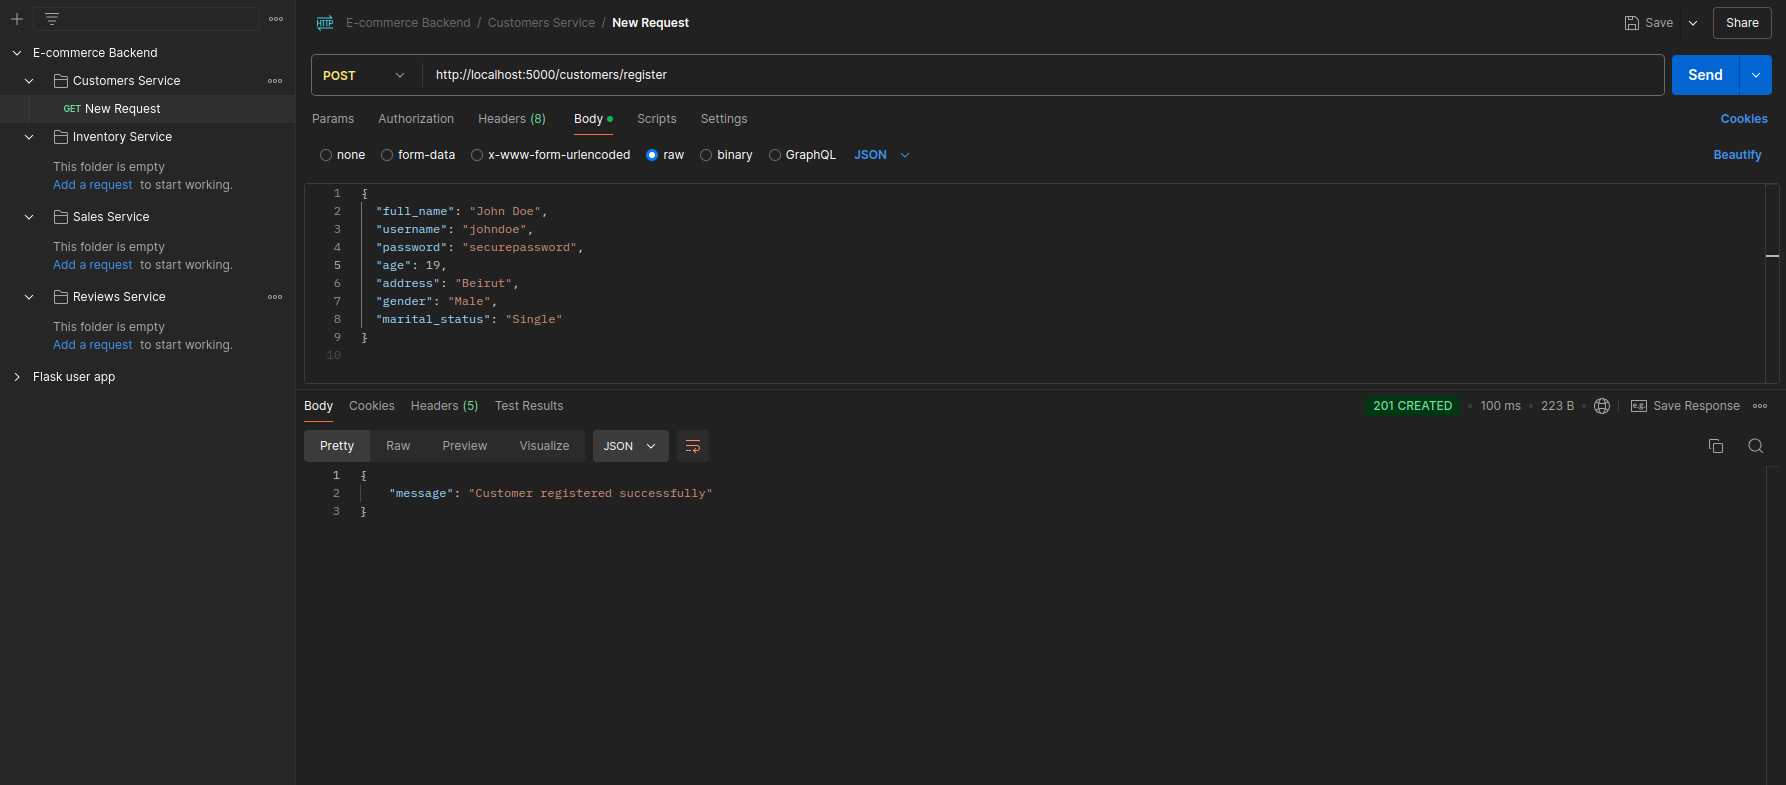
\includegraphics[width=0.9\textwidth]{images/3.png}
\caption{Customer registration}
\end{figure}
\begin{figure}[H]
\centering
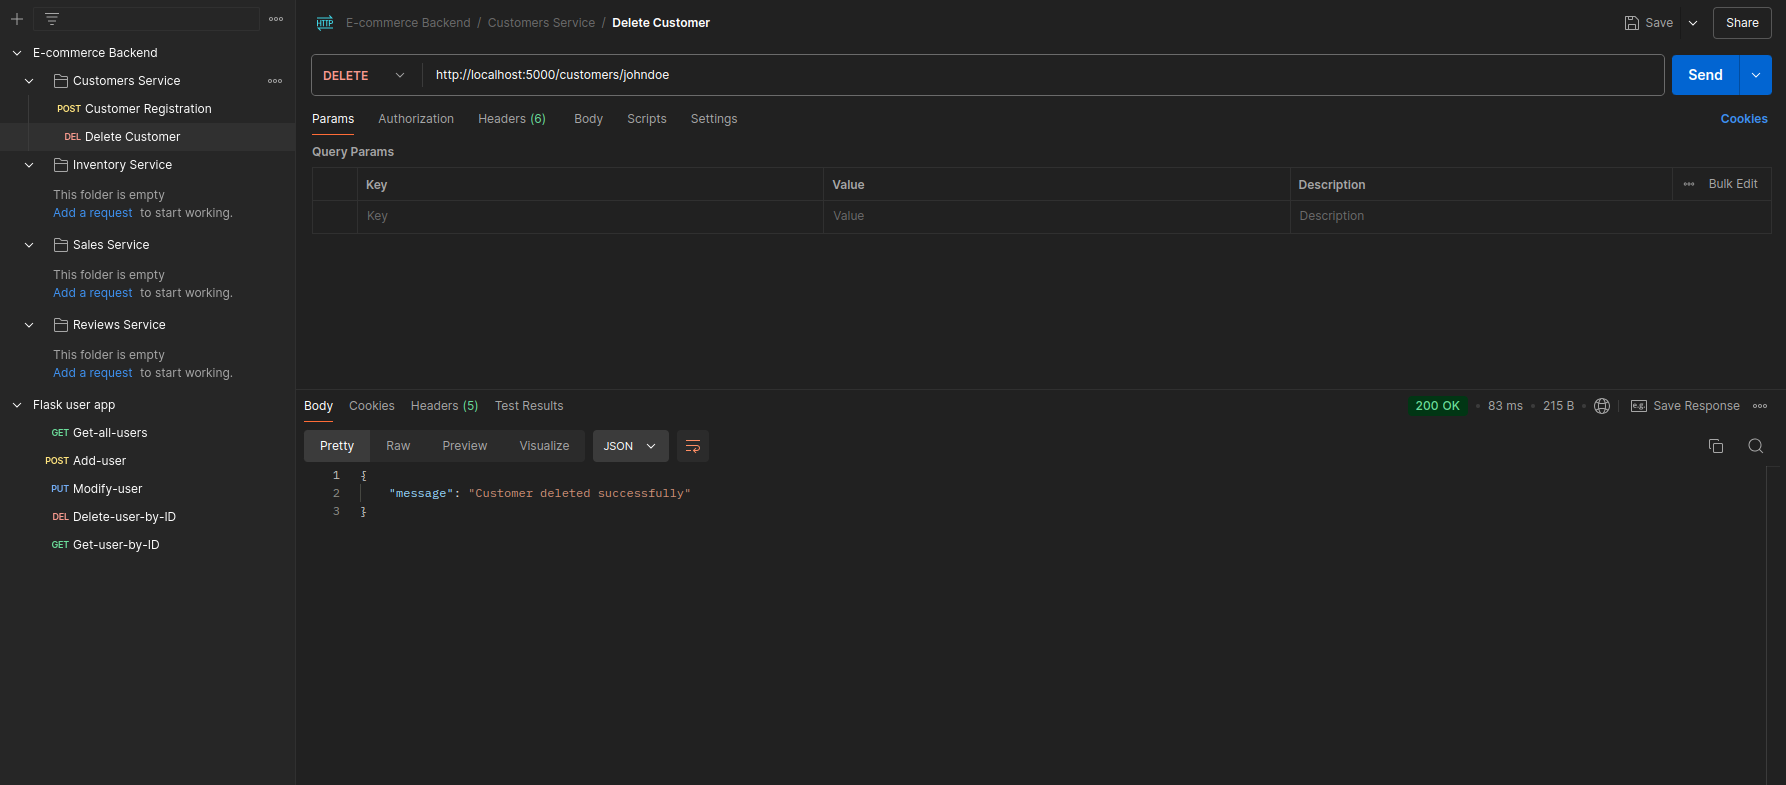
\includegraphics[width=0.9\textwidth]{images/4.png}
\caption{Delete customer}
\end{figure}
\begin{figure}[H]
\centering
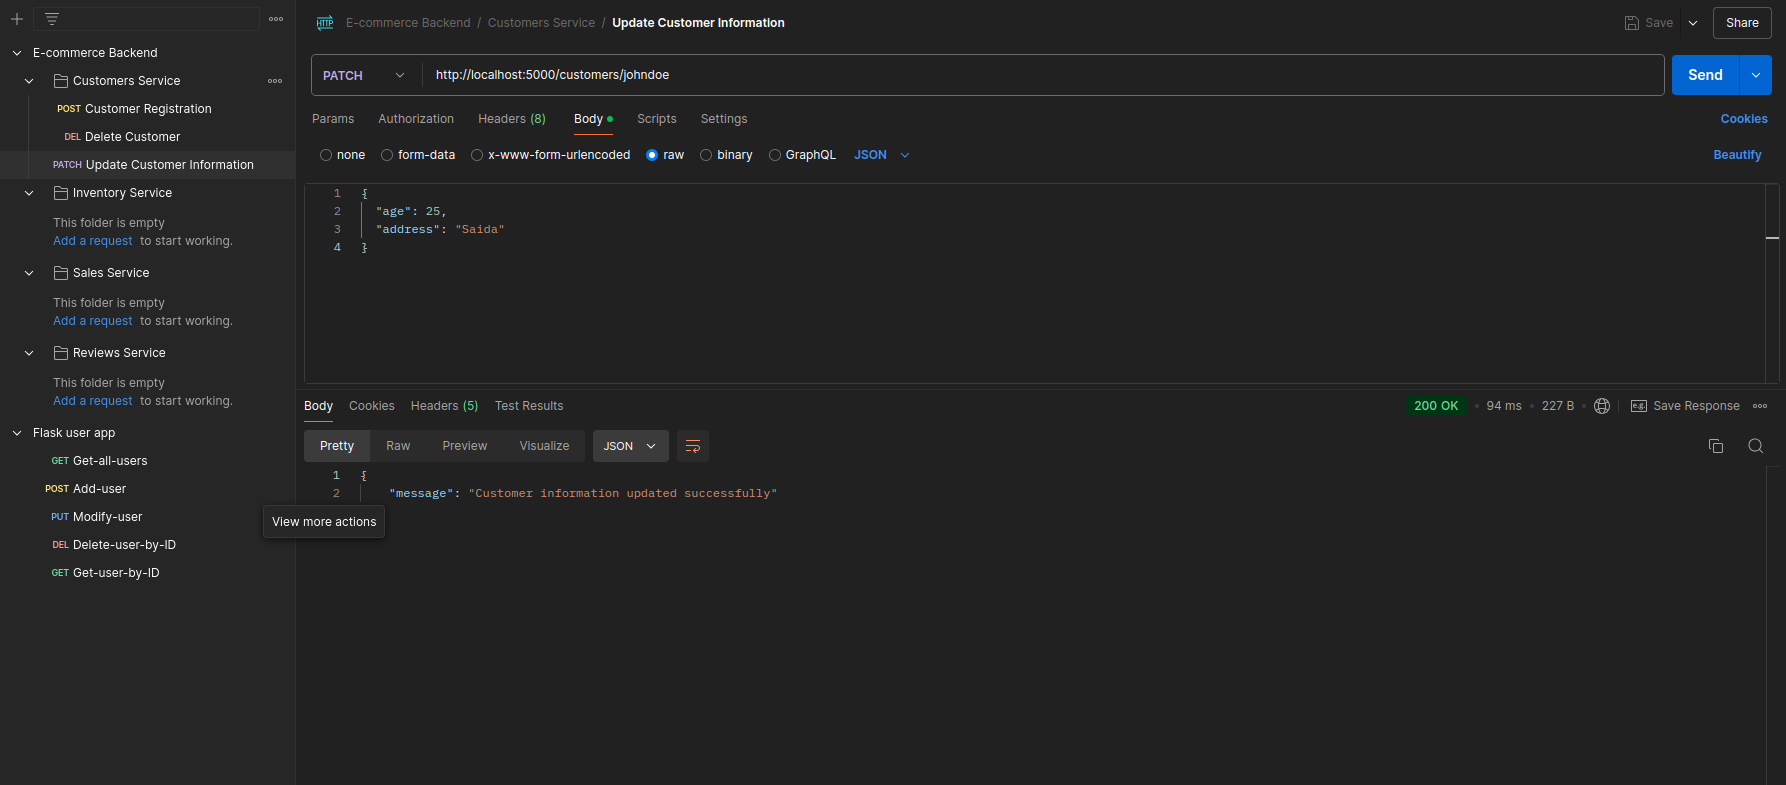
\includegraphics[width=0.9\textwidth]{images/5.png}
\caption{Update customer information}
\end{figure}
\begin{figure}[H]
\centering
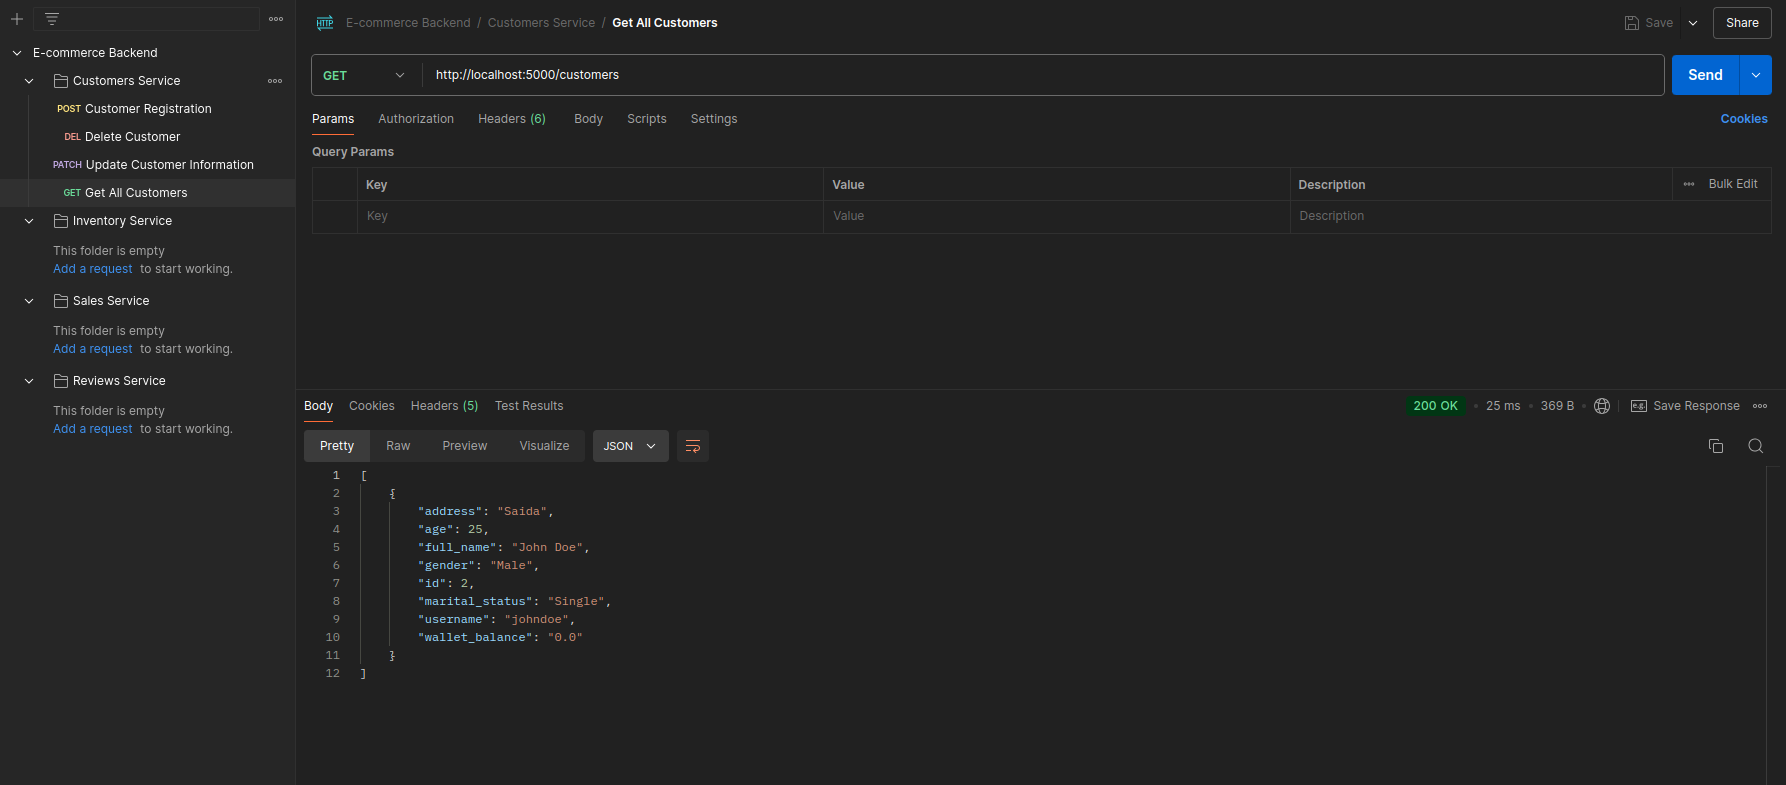
\includegraphics[width=0.9\textwidth]{images/6.png}
\caption{Get all customers}
\end{figure}
\begin{figure}[H]
\centering
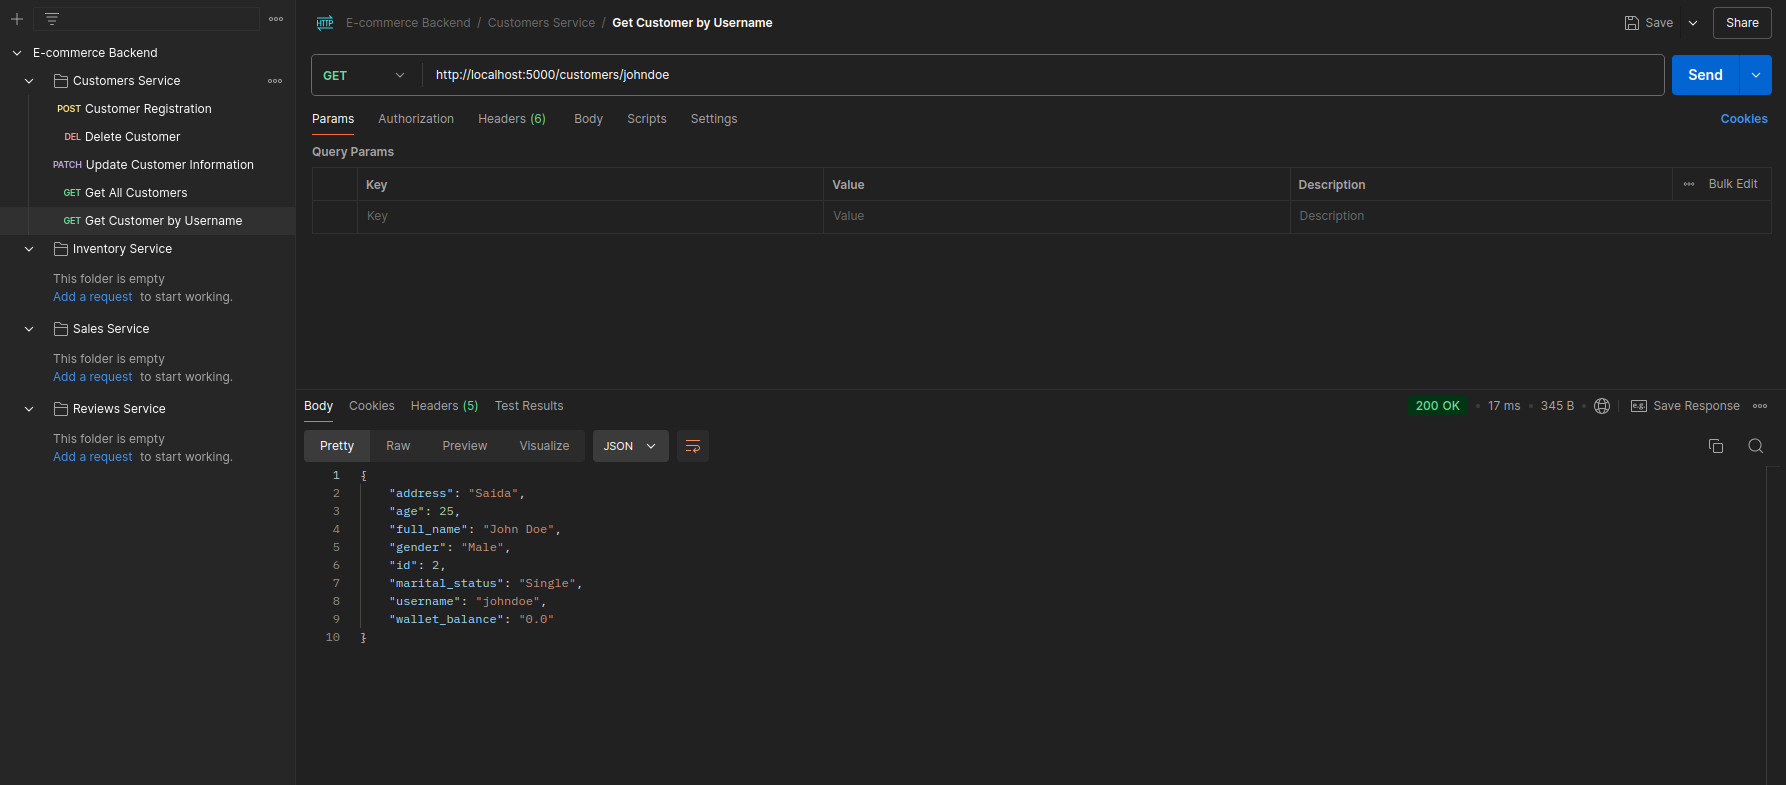
\includegraphics[width=0.9\textwidth]{images/7.png}
\caption{Get customer per username}
\end{figure}
\begin{figure}[H]
\centering
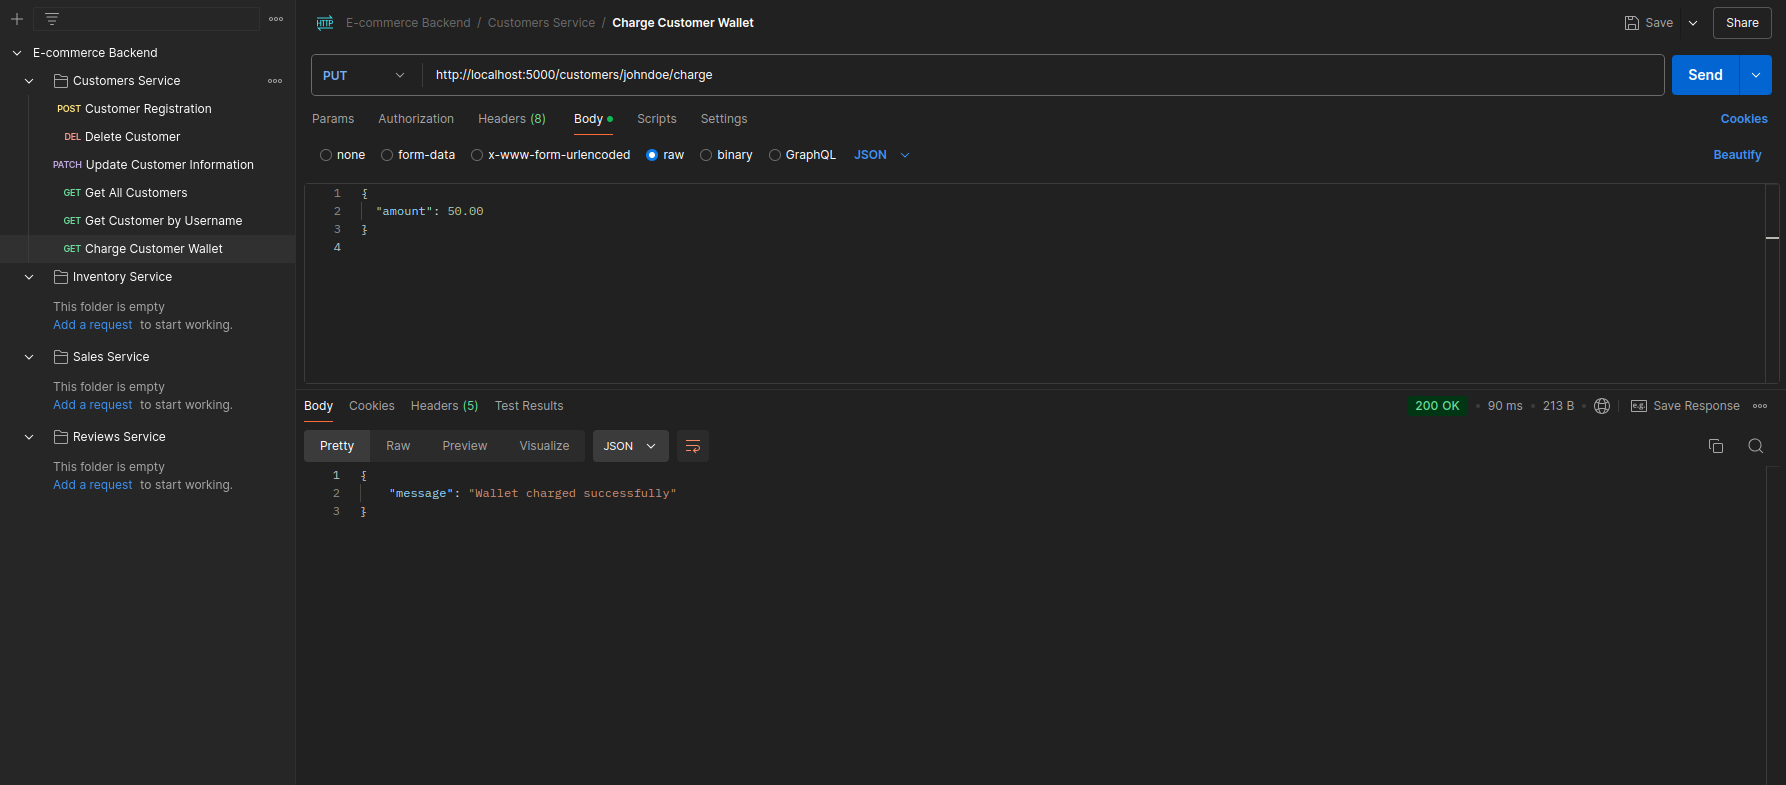
\includegraphics[width=0.9\textwidth]{images/8.png}
\caption{Charge customer wallet in dollars}
\end{figure}
\begin{figure}[H]
\centering
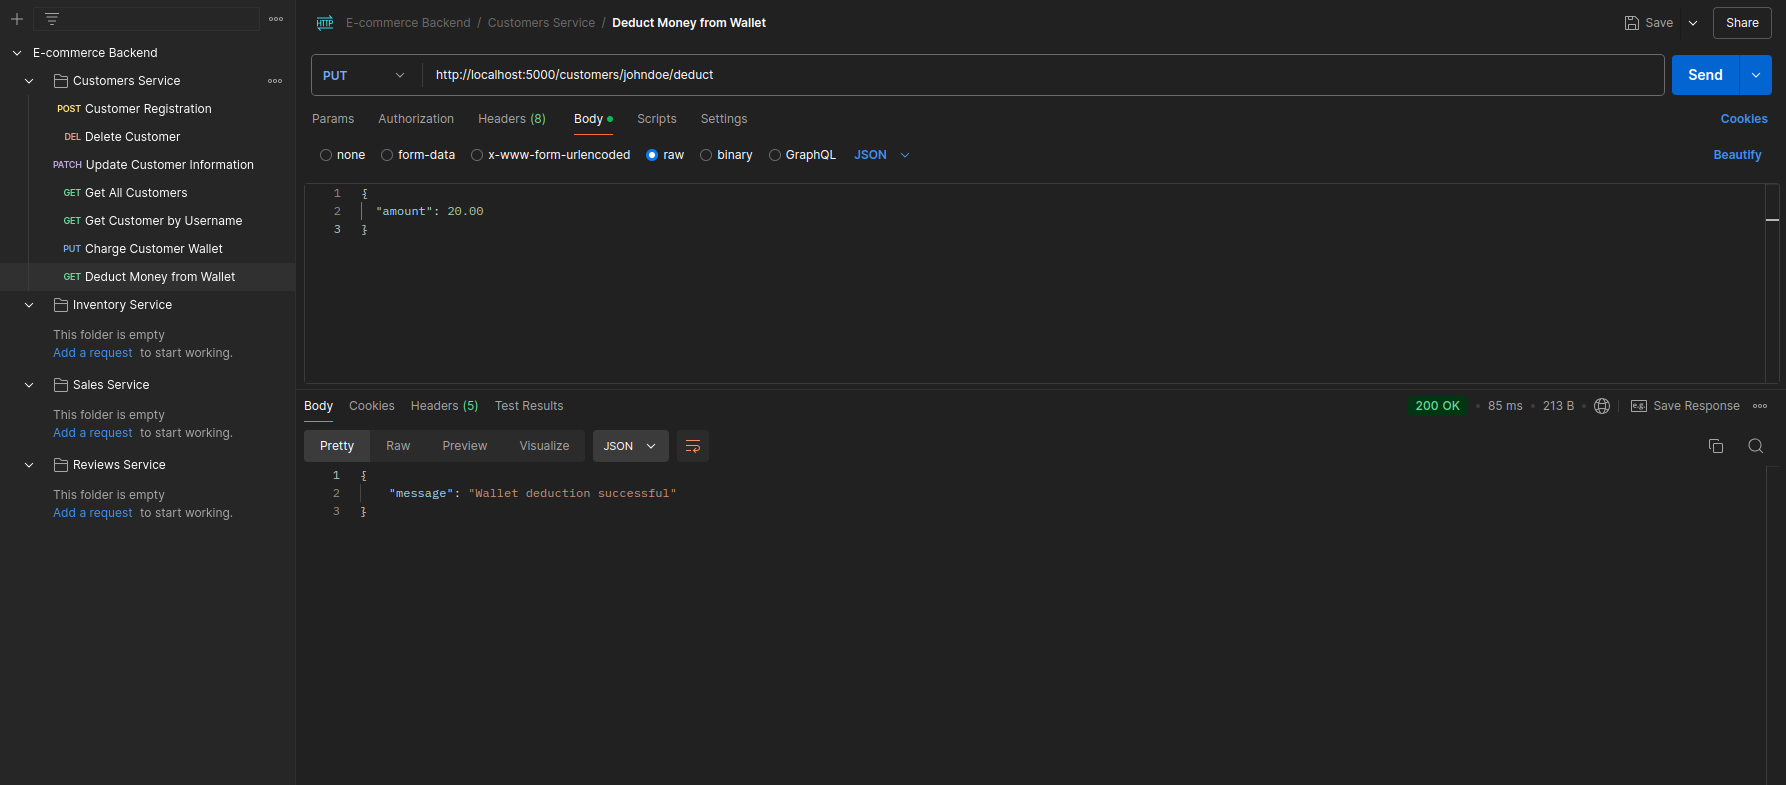
\includegraphics[width=0.9\textwidth]{images/9.png}
\caption{Deduct money from the wallet}
\end{figure}

\end{document}